
\documentclass[titlepage]{scrartcl}
\usepackage{enumitem}
\usepackage[british]{babel}
\usepackage[style=apa, backend=biber]{biblatex}
\DeclareLanguageMapping{british}{british-apa}
\usepackage{url}
\usepackage{float}
\restylefloat{table}
\usepackage{perpage}
\MakePerPage{footnote}
\usepackage{abstract}
\usepackage{graphicx}
% Create hyperlinks in bibliography
\usepackage{hyperref}

\usepackage[T1]{fontenc}
\usepackage[utf8]{inputenc}
\usepackage{blindtext}
\setkomafont{disposition}{\normalfont\bfseries}


\graphicspath{
    {./resources/},
}
\addbibresource{~/PerryPerrySource/LaTeX/DSP_Bibliography.bib}

\newsavebox{\abstractbox}
\renewenvironment{abstract}
  {\begin{lrbox}{0}\begin{minipage}{\textwidth}
   \begin{center}\normalfont\sectfont\abstractname\end{center}\quotation}
  {\endquotation\end{minipage}\end{lrbox}%
   \global\setbox\abstractbox=\box0 }

\usepackage{etoolbox}
\makeatletter
\expandafter\patchcmd\csname\string\maketitle\endcsname
  {\vskip\z@\@plus3fill}
  {\vskip\z@\@plus2fill\box\abstractbox\vskip\z@\@plus1fill}
  {}{}
\makeatother

\DeclareCiteCommand{\citeyearpar}
    {}
    {\mkbibparens{\bibhyperref{\printdate}}}
    {\multicitedelim}
    {}

\begin{document}
    \title{DSP Assignment 2\\Digital Audio Effects Implementation}
    \subtitle{\LARGE{Technical Report}}
    \author{Sam Perry\\U1265119}
    \date{}

    \begin{abstract}
        This report outlines the implementation, testing and evaluation of
        three real-time audio effects using the dsPIC 30F4013 digital signal
        processor.  Design choices, system specification, and final results
        are analysed.\\
        System specification is compared with alternative chips to understand
        the quality of the processor in relation to the state of DSP
        technology.\\
        Design choices are compared to choices made in previous work to outline
        the changes required to implement such effects outside unlimited
        resource systems.\\
        Final system performance is then discussed to determine further
        changes that could be made to improve performance.
    \end{abstract}

    \maketitle


    \section{Background/Literature:\\Digital Signal Processor/Microcontroller
    Overview}
    A digital signal processor (DSP) is a form of specialized microprocessor
    designed specifically for the processing of signals (such as audio signals
    in this case).~\parencite[p.11-12]{libtak2006ieh}. The DSP is used as part
    of a microcontroller that provides an interface for components such as
    Memory, data IO and peripherals that form the signal processing system.
    When considering the quality of a DSP system, there are many component
    specifications to consider, that contribute to the overall performance of
    the system. These include:
    \begin{itemize}
        \item CPU
        \item Memory
        \item System bus
        \item Bit depth
        \item Samplerate
        \item D/A \& A/D converters
    \end{itemize}

    In order to understand the specification of the
    dsPIC~\parencite{mt2004dspic} in relation to the standard of DSPs
    available, it will be compared to three other digital signal processors:
    \begin{itemize}
        \item Texas Instruments TMS320F2806~\parencite{ti2016pm}
        \item Freescale 56F8025~\parencite{fs2006dsc}
        \item Analog Devices ADSP-2126~\parencite{ad2012adsp}
    \end{itemize}

    \subsection{General Computing Factors}
    Factors such as memory and CPU speed affect all computing systems. These
    address the system's ability to perform calculations and handle data.

    \subsubsection{Memory}
    There are two types of memory that constitute the total memory of a
    microcontroller: program memory and data memory.

    \paragraph{Program Memory}~\\
    Most modern microcontrollers use flash memory for the storage of code
    executed at runtime. This is known as ROM (read-only memory) and may be
    reffered to as the ``program memory''. The size of this memory determines
    the amount of code that can be stored at any one time in the system.
    This has implications with regards to the complexity of the program, as
    insufficient program memory will limit the number of instructions that can
    be used for programming.~\parencite[p.317]{raf2014fdlm}

    \begin{table}[H]
    \centering
    \caption{DSP maximum available ROM memory}
    \label{my-label}
    \begin{tabular}{ll}
        \textbf{Model}     & \textbf{Program Memory}\\
        dsPIC30F4013/PIC24 & 48kb      \\
        TMS320F2806        & 256kb     \\
        56F8025            & 32kb      \\
        ADSP-2126          & up to 4mb
    \end{tabular}
    \end{table}

    These specifications indicate that the memory of the hardware used is
    relatively small compared to other devices available. This limits the
    complexity of programs that can be stored on the device. This accounts for
    the limited complexity of designs described in section \ref{design}.
    Clearly the ADSP has much more memory and has been designed for highly
    complex applications, however the TMS32F2806 series would also have
    sufficient memory for the programs designed in this task.


    \paragraph{Data Memory}~\\
    RAM (random-access memory) is volatile memory that is used for storing data
    used when executing instructions. Unlike ROM memory, RAM can be both read
    from and written to at runtime and is used for the storage of data that can
    change as instructions are executed. This is used for the storage of data
    such as audio buffers and parameter
    variables.~\parencite[p.317]{raf2014fdlm} The amount of RAM available
    determines the maximum size of data such as buffers for audio delays. The
    speed of the RAM is also integral to the overall performance of the system,
    as sufficient speed is required to read and write buffers as instructions
    are executed by the CPU (see section \ref{CPU})

    \begin{table}[H]
    \centering
    \caption{DSP maximum available RAM memory}
    \label{my-label}
    \begin{tabular}{ll}
        \textbf{Model}     & \textbf{RAM Size}\\
        dsPIC30F4013/PIC24 & 2kb      \\
        TMS320F2806        & 100kb     \\
        56F8025            & 4kb      \\
        ADSP-2126          & up to 2mb
    \end{tabular}
    \end{table}

    With the lowest memory of any processor in this comparisson, it is clear
    that the dsPIC is lacking in this area. This creates severe limitations in
    buffers and in the case of this project, resulted in severe delay line
    limitations. Again, the TMS32F2806 series would have a far more acceptable
    performance, allowing for multiple delays in a range of seconds as opposed
    to the small fractions of a second possible with the dsPIC.

    \subsubsection{System Bus}
    The system bus handles data IO between components such as the CPU
    and memory. For performance comparisson, the system bus's data width is
    used to determine the maximum amount of memory that the CPU is able to
    write to directly.~\parencite[p.318]{raf2014fdlm}
    For example a 16BIT system can support a maximum of $2^{16}$ memory
    addresses. This equals a maximum memory size of 64Kb of memory directly
    accessible by the CPU. However, a 32BIT system can support $2^{32}$ memory
    addresses which results in
    {\raise.17ex\hbox{$\scriptstyle\mathtt{\sim}$}}4GB of potential
    memory.~\parencite[p.34]{sd2006mfes}\\
    (When analysing specifications of DSP systems it is important not to
    confuse the processing architechuture with the bit depth of the DSP
    components as they affect different aspects of the system.)

    \begin{table}[H]
    \centering
    \caption{DSP bus architecture}
    \label{my-label}
    \begin{tabular}{ll}
        \textbf{Model}     & \textbf{Architecture Type}\\
        dsPIC30F4013/PIC24 & 16BIT      \\
        TMS320F2806        & 32BIT     \\
        56F8025            & 16BIT      \\
        ADSP-2126          & 32/40BIT
    \end{tabular}
    \end{table}

    The bus architecture is largely dictated by the total amount of memory
    available to the system and this is reflected in the specification shown in
    the table above. A 16BIT architecture is expected, given the 2kb of memory
    supported by the dsPIC and is marginally faster than higher bit
    architectures as there are less memory locations to allocate. 

    \subsubsection{CPU}\label{CPU}
    The CPU (Central Processing Unit) is the component that executes
    instructions and performs calculations on data. The speed at which the CPU
    can execute instructions and store results is critical to the performance
    of the system.

    \paragraph{Clock Speed}~\\
    Measured in cycles per second (Hz), the clock speed defines the number of
    calculations that can be performed per second. A higher clock speed
    indicates a higher number of calculations performed per second. This is
    particularly significant in realtime DSP application as a sufficient number
    of calculations must be performed in a set period of time in order to
    process audio as quickly as it is provided to the system.  If the clock
    speed is not sufficient, this may result in instructions being missed due
    to an interrupt before the processor has been able to complete them. This
    can create artefacts in output audio.~\parencite[p.34]{sd2006mfes}\\

    It should be noted that this is not an entirely accurate measurement for
    speed as different manufacturers have different definitions of a
    ``calculation''.~\parencite[p.3-4]{bdti2000cdp} For a more accurate
    representation, an impartial benchmark from BDTI has been included where
    possible.~\parencite[p.1]{bdti2013pg}
    \begin{table}[H]
    \centering
    \caption{DSP CPU clock speed}
    \label{my-label}
    \begin{tabular}{lll}
        \textbf{Model}              & \textbf{CPU Clock Speed}
                                    &\textbf{BDTI(sim)mark2000\textsuperscript{TM}}\\
        dsPIC30F4013/PIC24 & 70MHz              & 190\\
        TMS320F2806        & 90MHz              & n/a\\
        56F8025            & 80MHz              & 110\\
        ADSP-2126          & 200MHz             & 1090\\
    \end{tabular}
    \end{table}
    From this, it can be seen that the dsPIC and 56F8025 perform significantly
    worse than the ADSP. This has a negative impact on samplerate as it must be
    lowered to account for the lack of processing power. A sample rate of 8Khz
    was used as opposed to the 44.1Khz samplerate that would be feasable on the
    ADSP processor.

    \paragraph{Architecture}~\\
    The CPU architecture refers to the design of memory units and bus layouts.
    The most common designs are von Neumann and Harvard architectures. The von
    Neumann architecture combines program and memory data, allowing only serial
    access of memory. By seperrating program and data memory, the Harvard
    architecture allows for simulataneous access of data and program memory,
    making it the more efficient of the two designs.~\parencite[p.320-321]{raf2014fdlm}
    \begin{figure}[H]
        \caption{von Neumann CPU architecture~\parencite[p.320]{raf2014fdlm}}
        \makebox[\textwidth]{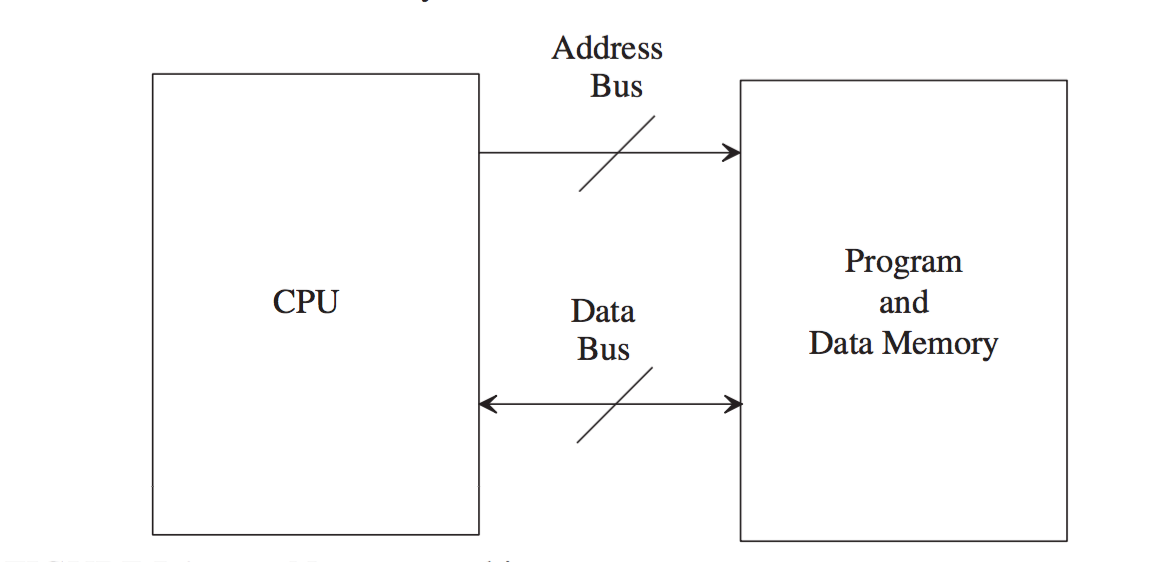
\includegraphics[width=0.75\textwidth]{neumann}}
    \end{figure}
    \begin{figure}[H]
        \caption{Harvard CPU architecture~\parencite[p.321]{raf2014fdlm}}
        \makebox[\textwidth]{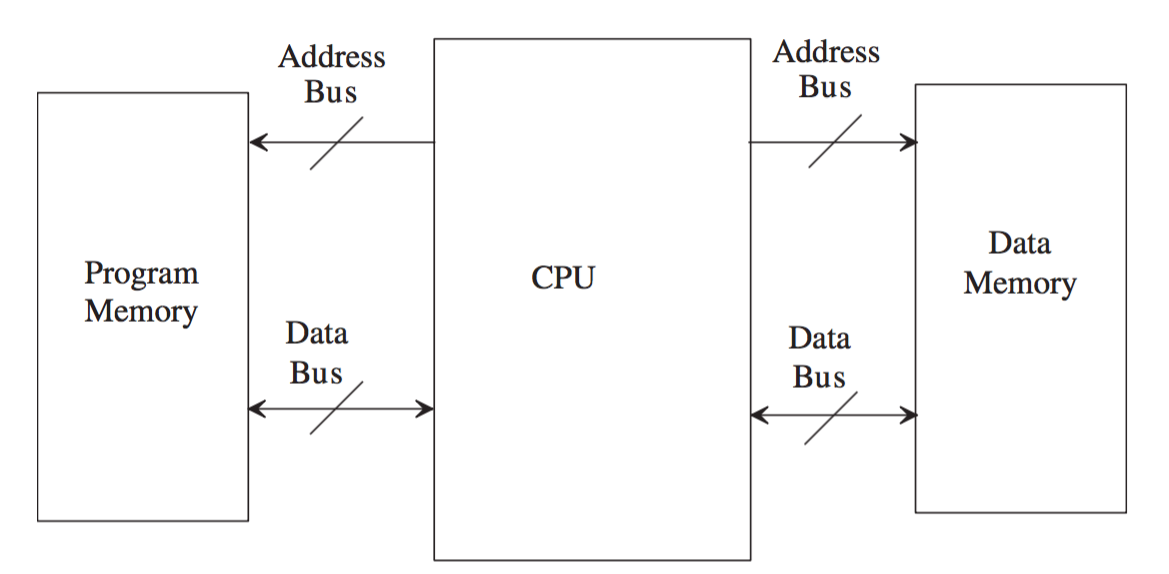
\includegraphics[width=0.75\textwidth]{harvard}}
    \end{figure}

    \begin{table}[H]
    \centering
    \caption{DSP bus architecture}
    \label{my-label}
    \begin{tabular}{ll}
        \textbf{Model}              & \textbf{Architecture Type}\\
        dsPIC30F4013/PIC24 & Modified Harvard\\
        TMS320F2806        & Harvard\\
        56F8025            & Dual Harvard\\
        ADSP-2126          & Super Harvard
    \end{tabular}
    \end{table}

    Most modern DSPs use variations on the Harvard architecture for it's
    performance. Variations of this have been used in all examples.

    \section{DSP Specific Factors}
    DSP specific factors relate to components specifically affecting the system's
    ability to handle audio signals. These will determine the quality of audio
    manipulation and affect the computational requirements for the system. This
    section briefly covers the computational impact of the DSP specific
    factors.

    \subsection{A/D \& D/A Converters}
    A/D and D/A converters are required for audio input and output. Depending
    on the microcontroller used, these may be integrated in the main circuit
    board or available as peripherals that can be attached via ports (as is the
    case for the PIC24 board used). The quality and accuracy of these
    converters will clearly have an effect on the audio output and using
    converters that can perform as transparently as possible is essential for a
    high quality system.~\parencite[p.147-152]{kadis2012sosr}
    
    \subsubsection{Samplerate}
    The samplerate defines the frequency at which a measurement will be taken
    from the input audio. This is significant due to the quantity of
    information returned from the A/D converter for processing. Higher sample
    rates generate more measurements per second and thus require more values
    to be computed per second as discussed in section \ref{CPU}
    \begin{figure}[H]
        \caption{Illustration of sine wave sampling~\parencite[p.140]{kadis2012sosr}}
        \makebox[\textwidth]{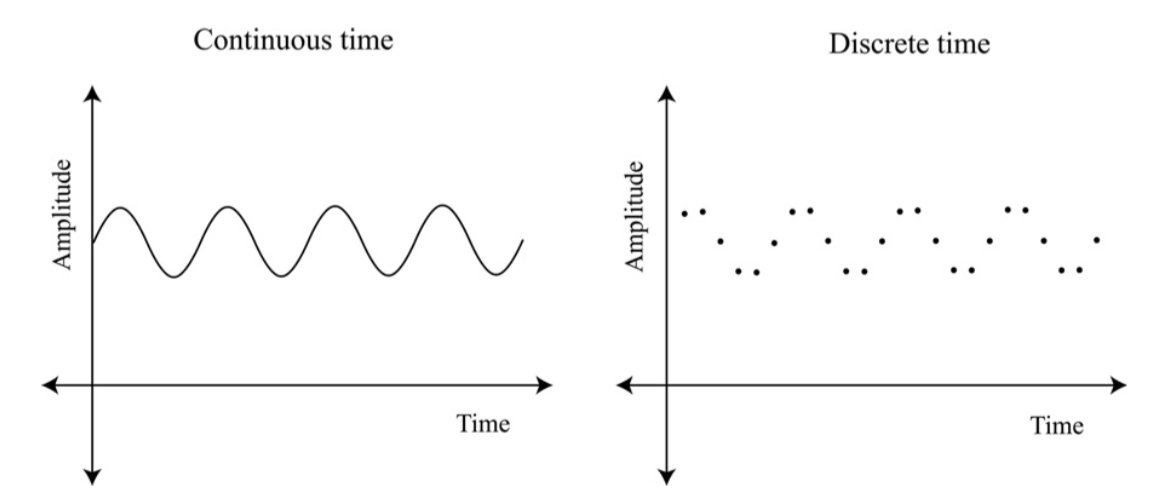
\includegraphics[width=\textwidth]{quantization}}
    \end{figure}
    \begin{figure}[H]
        \caption{Illustration of quantization error resulting from a low sample
        rate.~\parencite[p.146]{kadis2012sosr}}
        \makebox[\textwidth]{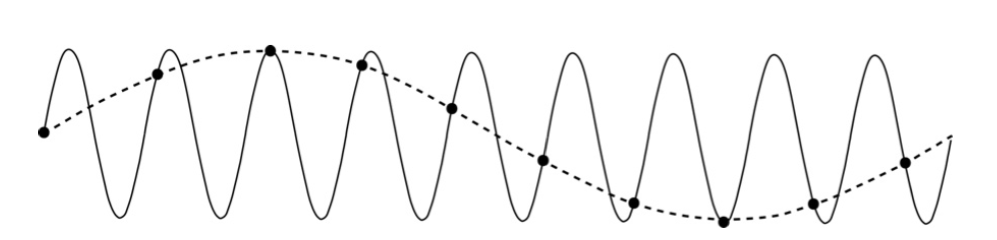
\includegraphics[width=\textwidth]{sampling_error}}
    \end{figure}

    \subsubsection{Bit Depth}
    The audio bit depth determines the accuracy to which amplitudes can be
    differentiated. Higher bit depths result in a higher dynamic range in the
    signal. This has implications for the converters as higher bit rates
    require higher accuracy in generating values for each sample.~\parencite[p.143-145]{kadis2012sosr}

    \section{Design/Analysis}\label{design}
    Effect implementation was largely dicatated by the limitations of the
    dsPIC. As the device had severe memory and processing limitations, it was
    not possible to create effects to the standard of the first assignment. As
    a result, effects were created to emulate the perceptual effect of an echo,
    reverb and chorus under these limitations.

    \subsection{Echo}
    The echo was implemented using a single tap FIR filter. This was intended
    to maximise available memory for the delay time. Through stripping out all
    unnessesary features, a maximum delay size of 700 samples was acheived with
    the addition of two UI switches that could be used for increasing and
    decreasing delay size at runtime.  At a samplerate of 8Khz, this allowed
    for a single delay of \textgreater50ms (93.750ms) defined as the minimum
    for the definition of an echo
    by Z{\"o}lzer~\citeyearpar[p.]{zolzer2011dafx}

    \begin{figure}[H]
        \caption{Echo example}
        \makebox[\textwidth]{\includegraphics[width=0.4\textwidth]{echo_measure}}
    \end{figure}

    \subsection{Chorus}
    Three delays of variable size were used to emulate the multi-instrument
    effect created by a chorus. This created three phase shifted versions of
    the original signal which created the perception of multiple instruments.
    The delay time modulation was not possible due to the computational power
    required to implement a modulated delay line on a sample by sample basis.

    \subsection{Reverb}
    The reverb implementation involved a combination of an FIR and IIR filter,
    as defined by Z{\"o}lzer~\citeyearpar{zolzer2011dafx}. This performed
    poorly when compared to the moorer reverb structure used in assignment 1,
    however the complexity of such a structure would require superior
    performance in almost all aspects of the system.
    The design used created a delayed echo that could act as a crude reverb.

    \subsection{User Interface}
    The UI was designed using eight switches and the LCD to create a
    navigatable menu that can be used for the selection of effect, effect
    parameters and volume control. The effect parameter menu is able to update
    it's items dynamically based on the active effects. The desired effect can
    then be selected by cycling through, using repeated presses of the effects
    menu button. Parameter variables can then be increased and decreased for
    the selected effect using two switches.\\
    It was not possible to use the UI in conjunction with any actual audio
    effect as the UI would need to be processed after any audio effects. in
    practice this caused problems as the program did not always have time to
    complete UI logic before the interupt, causing graphical errors and
    unexpected results. As a result, the project presented is a prototype to
    demonstrate possibilities given a capable system.

    \section{Results}
    Overall, the results produced were not of a high standard. The low signal
    to noise ratio, low sample rate and over-simplification of designs made it
    impossible to create results usable in a professional context. With a
    sample rate of 8Khz, a cutoff sampling frequency of 4000khz was created.
    This resulted in a telephony frequency response that removed higher
    frequencies due to the low nyquist rate. Poor converters added significant
    noise to the output which further degraded results. However, steps were
    taken to create the best quality outcome with the resources available.

        \subsection{Echo}
        A maximum single tap delay of 750 samples was achieved through the
        stripping of all unnecessary components. Without a visual UI,
        this was controlled through the use of two switches that
        incremented/decremented the delay in values of 10 samples every 100ms. 
        The lack of a feedback loop resulted in a very simplistic delay with
        equally simplistic results in terms of perception. A feedback was not
        implemented to differentiate this from the reverb design.


        \subsection{Chorus}
        The implementation provided a perceptually similar alternative to the
        infeasible modulated delay line design from the previous assignment.
        Each delay can be set to up to a maximum delay time of 250 samples.
        This allows for manual shifting of phases to taste. Overall this
        results in a functional alternative at the cost of perceptual quality.
        Through the use of a spectrogram, it can be seen in figure
        \ref{fig:cho_spec} that the signal is clearly noisy and distorted with
        harmonics produced far above the nyquist rate. This is most likely due
        to the poor converter performance
        \begin{figure}[H]
            \caption{Chorus spectrogram displaying distortion}
            \makebox[\textwidth]{\includegraphics[width=\textwidth]{Chorus_spectrogram}}
            \label{fig:cho_spec}
        \end{figure}

        \subsection{Reverb}
        A crude slapback reverb was created using an FIR/IIR filter
        combination. The result was a short reverb tail with decaying
        repetitions of the dry sample. This would have been vastly improved
        with the addition of further parallel comb filters or all pass filters.
        A clear decaying echo can be see in figure \ref{fig:rev_wav}

        \begin{figure}[H]
            \caption{Reverb waveform}
            \makebox[\textwidth]{\includegraphics[width=\textwidth]{Click_reverb_waveform}}
            \label{fig:rev_wav}
        \end{figure}
        
    \section{Further Work}
    Building on skills learnt in this project, results could be improved
    significantly through the use of C code directly, allowing for greater
    control over the underlying logic than is possible through Flowcode. This
    would also offer greater scope for design as it would no longer be limited
    to the relatively limited Flowcode macros.\\
    The main improvement would be to use a more capable system. It is clear
    that the limitations of the system have impeded the quality of results to
    an unreasonable degree. 

    \section{Conclusions}
    Overall this project has offered insight into the performance issues and
    limitations involved when programming for integrated systems of finite
    resources. It has also highlighted the limitations of real-time processing
    as opposed to offline processing.\\
    When planning a hardware system it is clear that the system specification
    and design of it's code must be as efficient as possible in order to
    produce the quality of results that are possible on unlimited resource
    systems such as a standard computer.
    \printbibliography

\end{document}
